\documentclass{article}
\usepackage[utf8]{inputenc}

\title{Two Dimensional Hydrodynamics and Simulating Acoustic Bessel Waves in a Fluid}
\author{Mohammed Abdelaziz}
\date{December 16 2016}

\usepackage{natbib}
\usepackage{graphicx}
\usepackage{titlesec}
\usepackage{ amssymb }
\usepackage{amsmath}
\usepackage{verbatim}



\titleformat{\section}[runin]
  {\normalfont\Large\bfseries}{\thesection}{1em}{}
\titleformat{\subsection}[runin]
  {\normalfont\large\bfseries}{\thesubsection}{1em}{}
  
\begin{document}

\maketitle
\section{Background and Motivation}

Acoustic tweezing is an effect by which objects in the path of an acoustic wave's propagation may experience a force toward the source rather than away from it. For acoustic Bessel beams there is a specific mechanism by which this can occur. The beam, which has an intensity profile of a zeroth-order Bessel function, has the unique property that it is self-healing. This means if an object is in its path, the beam diffracts and is then reformed on the other side of the object. It has been shown that for certain properties of the object and beam, this process causes a net force on the object in the direction opposite the beam's propagation.

This project worked toward the goal of simulating this acoustic tweezing effect by simulating acoustic Bessel waves travelling through a fluid in the absence of other objects inside the fluid.  
\section{Methods}
The problem of interest is the propagation of a wave with an intensity profile of a radial zeroth order Bessel function $J_0(k_r r)$ with radial wavenumber $k_r$ through some three-dimensional volume. If we take the direction of propagation to be along the $z$-axis, then the problem is axisymmetric, and we can switch from using cylindrical coordinates to looking at a two-dimensional slice of the volume at constant azimuthal angle $\phi$, with a horizontal axis going from $0$ to $r$ and a vertical axis from $0$ to $z$. In two-dimensions, the Bessel function is symmetric about $r=0$, so we can switch to Cartesian coordinates and view the horizontal axis from $-x$ to $x$, in the $y=0$ plane, to be able to observe effects at the center of the Bessel function as well as to either side of it.

A two-dimensional hydrodynamics code was written as an extension from a previously coded one-dimensional version. It follows from the continuity equations that we can construct a vector of four conserved variables: $$ \vec U = (\rho, \rho v_x, \rho v_y, E) $$ which will change due to horizontal fluxes by the vector $$\vec F = \big(\rho v_x, \rho v_x^2+ P, \rho v_x v_y, (E + P) \rho v_x\big)$$ and due to vertical fluxes by $$ \vec G = \big(\rho v_y , \rho v_x v_y, \rho v_y^2 + P, (E + P) \rho v_y \big)$$ Here, $\rho$ is the mass density of a fluid element, $v_i$ is the $i$-velocity of that fluid element, $E$ is the energy density of it, and $P$ is its pressure. Thus the entries of $\vec U$ correspond, respectively, to conservations of mass, $x$-momentum, $y$-momentum, and energy. At every time step, the change in these conserved quantities is computed as 
$$ \frac {d \vec U_{i,j}}{dt} = L(\vec U) = - \frac{\vec F_{i+1/2,j} - \vec F_{i-1/2,j}}{\Delta x} - \frac{\vec G_{i,j+1/2}-\vec G_{i,j-1/2}}{\Delta y}$$ for horizontal cell index $i$ and vertical cell index $j$. A second-order spatial interpolation method was used to compute the cell states on either side of an interface (left and right of the interface for horizontal flux, or above and below the interface for vertical flux). The HLL Riemann solver was then applied to these states to calculate the fluxes. It is useful to calculate the speeds involved in each cell:
$$\lambda^\pm = v \pm c_s$$ for sound speed $c_s = \sqrt{\gamma P/\rho}$, where $\gamma$ is the adiabatic index of the fluid, taken to be $1.4$ for ideal gases. Then  the values $\alpha^\pm$ defined as $$\alpha^\pm = \text{MAX} (0,\pm \lambda^\pm(\vec U^L), \pm \lambda^\pm (\vec U^R))$$ are used to compute the flux through the interface:
$$ F^{HLL} = \frac{\alpha^+ \vec F ^L + \alpha^- \vec F^R - \alpha^+ \alpha^- (\vec U^R - \vec U^L)}{\alpha^+ + \alpha^-}$$ Where L denotes the state to the left of the interface, and R the state to the right. In a first order spatial scheme, these cell states are straightforwardly the values at the cell centers on either side of the interface. In the second order interpolation method, a piecewise linear method is used to compute these L and R states based on an additional cell on each side of the cells that would have been used in the first order method. Specifically, for an interface labelled $i+1/2$ which is between cells $i$ and $i+1$, and denoting any entry of $\vec U$ as $c$, the state just to the left of the interface is 
$$c^L_{i+1/2} = c_i + 0.5 \ \text{minmod}(\theta(c_i - c_{i-1}), 0.5 (c_{i+1} - c_{i-1}, \theta (c_{i+1} - c_i))$$ while the state just to the right is 
$$c^R_{i+1/2} = c_{i+1} - 0.5 \ \text{minmod}(\theta(c_{i+1} - c_i), 0.5(c_{i+2} - c_i), \theta(c_{i+2} - c_{i+1}))$$ The minmod function is defined
$$\text{minmod} (x,y,z) = \frac{1}{4} |\text{sgn}(x) + \text{sgn}(y)| (\text{sgn}(x) + \text{sgn}(z)) \text{min} (|x|,|y|,|z|)$$ and the parameter $1 \leq \theta \leq 2$ controls the diffusivity of the interpolation. $\theta = 1.5$ was used for this project. These equations are sufficient to compute the horizontal flux at each timestep. The equations for the vertical flux are completely analogous, with the states $L$ and $R$ being replaced by up and down states $U$ and $D$. With both fluxes calculated, $L(\vec U)$ can be computed, and Shu and Osher's third-order Runge-Kutta method can be used for time integration:
\begin{align*}
    \vec U ^{(1)} &= \vec U ^n + \Delta t L(\vec U^n) \\
    \vec U ^{(2)} &= \frac{3}{4} \vec U^n + \frac{1}{4} \vec U^ {(1)} + \frac{1}{4} \Delta t L(\vec U^{(1)}) \\
    \vec U ^{n+1} &= \frac{1}{3} \vec U^n + \frac{2}{3} \vec U^{(2)} +\frac{2}{3} \Delta t L(\vec U^{(2)}) \\
\end{align*}
for computing $\vec U$ at time step $n+1$ from time step $n$. Finally, the Courant condition for two dimensional hydrodynamics is $$C = \frac{\text{MAX}(\alpha_x^\pm) \Delta t}{\Delta x} + \frac{\text{MAX}(\alpha_y^\pm) \Delta t}{\Delta y} \leq 1 $$

The time step was computed according to this condition for a chosen CFL number of $C = 0.7$ at each step. Thus numerical instabilities were avoided by calculating $\Delta t$ adaptively. 
\section{Qualitative Tests}
The two-dimensional hydrodynamics code can be tested for the correct qualitative behavior in a number of ways. The selected methods were to see what results the code produces for the problems of Kelvin-Helmholtz instability and a corner implosion.

The initial conditions for both tests were chosen based on the work of Jonathon Zrake, who has published plots for these, so that the qualitative behavior of the simulations could be compared to known results.
\subsection{Kelvin-Helmholtz Instability}
In Kelvin-Helmholtz instability, a fluid is initialized with two or more regions of different densities, and an initial velocity field such that there is a shear velocity present at the boundary between different density zones. The pressure was initialized to be a uniform $P_0$ throughout the fluid, while the density was defined continuously but formed three distinct regions in $0 \leq x \leq L/4$, $ L/4 \leq x \leq 3L/4$, and $ 3L/4 \leq x \leq L$, given a total square region of size $L \times L$. The vertical velocities were defined in a similar way, and the horizontal velocity oscillates along the $y$-direction for two wavelengths of a selected amplitude $\omega_0 = 10^{-1}$. The exact initial conditions are:
$$\begin{pmatrix} \rho \\ P \\ v_y \\ v_x \end{pmatrix}
 = \begin{pmatrix}\frac{\rho_2 - \rho_1}{2} \left( \tanh \frac{x-L/4}{\delta} - \tanh \frac{y - 3L/4}{\delta} \right) + \rho_1 \\
 P_0 \\
 \frac{v_{y2} - v_{y1}}{2} \left( \tanh \frac{x-L/4}{\delta} - \tanh \frac{y - 3L/4}{\delta} -1 \right) \\
 \omega_0 \sin{4 \pi y}\end{pmatrix}$$ for $P_0 = 2.5$, $\rho_1 = 1.0$, $\rho_2 = 2.0$, $v_{y1} = -0.5$, $v_{y2} = 0.5$, and $\delta = 0.035$ in a square of length $L = 1.0$. Periodic boundary conditions were applied in the $y$-direction, so that ghost cells in the minimum and maximum $y$ zones were computed as an average of the first and last rows real cells at $y = 0$ and $y=1$. In the $x$-direction, standard fixed boundary conditions were used, so that the columns of ghost cells retained their cell values for the duration of the simulation. Density plots of the initial condition and a step after some time evolution are shown in Figure \ref{f:kh}. The system develops vortices, as expected.
 
 \begin{figure}
     \centering
     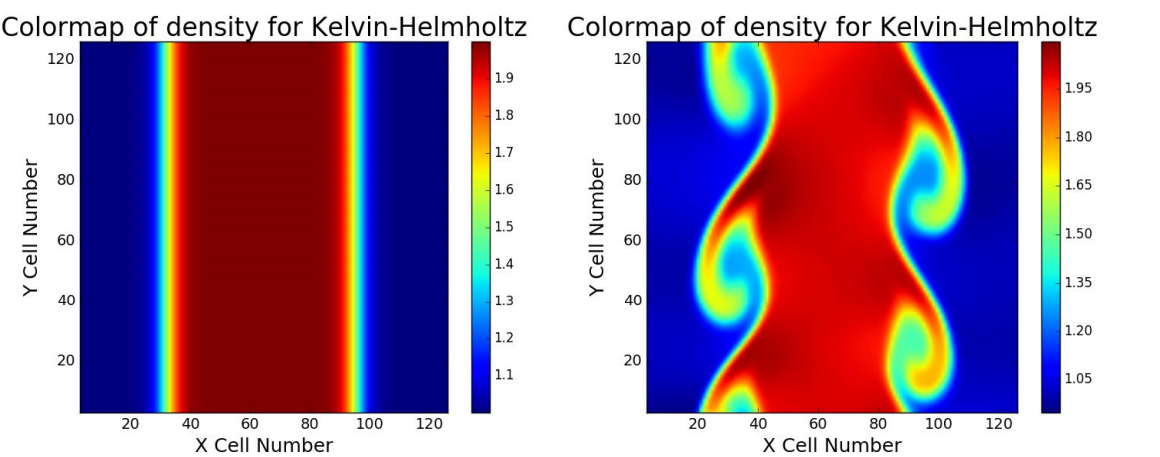
\includegraphics[width=\textwidth]{figKH.png}
     \caption{Initial condition and time evolution of a Kelvin-Helmholtz instability}
     \label{f:kh}
 \end{figure}
\subsection{Corner Implosion}
In the second qualitative test, the system is initialized, again in a square of length $L=1$, to have two distinct regions as follows:
\begin{align*}
    x + y &> L/2 & x+y &\leq L/2 \\
    \rho &= 1 & \rho &= 0.125 \\
    P &= 1 & P &= 0.140 \\
\end{align*}
and zero velocity everywhere. As the system evolves, the higher density region moves toward the $x=0$, $y=0$ corner, and forms a shockwave back outward due to reflecting boundary conditions (fluid elements at the border of the $L \times L$ square with velocities oriented toward a ghost cell have the appropriate component of their velocity reversed). 

This test helps check that the code resolves diagonal motion appropriately. The system should be symmetric about the line $y=x$ throughout the entire evolution, and this result was obtained. Figure \ref{f:ci} shows a density plot of the system shortly after the initial reflection occurs, and the entire time evolution can be seen in an accompanying video file.

 \begin{figure}
     \centering
     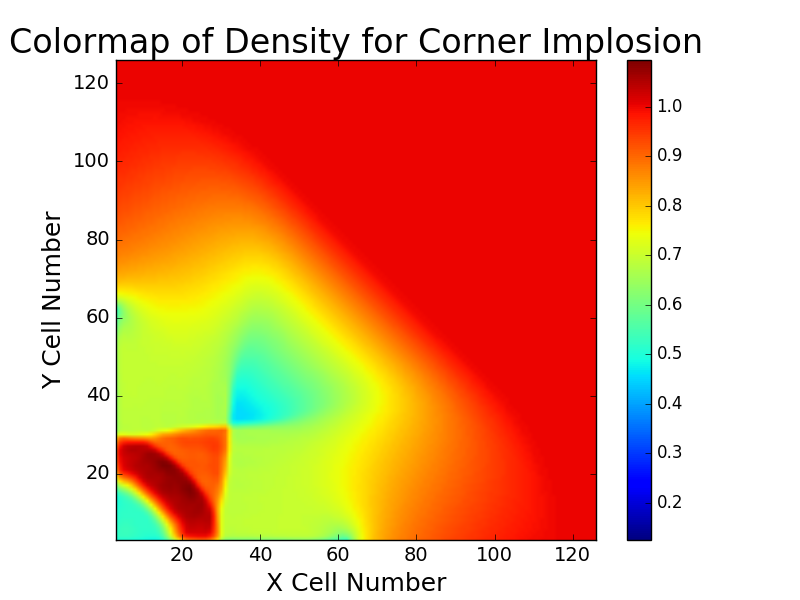
\includegraphics[width=0.75\textwidth]{figCI.png}
     \caption{Density plot of the corner implosion just after reflection from the corner}
     \label{f:ci}
 \end{figure}
 
\section{Convergence Test}
To test for quantitative behavior in addition to the above qualitative tests, and isentropic wave was initialized and allowed to run.

The wave was initialized with:
\begin{align*}
    f(x,y) &= \left(1 - \left( \frac{x-x_0}{\sigma}\right)^2 - \left( \frac{y-y_0}{\sigma}\right)^2 \right)^2  \ \ |x-x_0| < \sigma \ \text{and} \ |y-y_0| < \sigma\\
    \rho(x,y) &= \rho_0 (1 + \alpha f(x,y)) \\
    P(x,y) &= P_0 \left( \frac{\rho}{\rho_0} \right)^\gamma \\
    v(x,y) &= \frac{2}{\gamma-1} \left(\sqrt{\frac{\gamma P}{\rho}} - \sqrt{\frac{\gamma P_0}{\rho_0}}\right) \\
    \rho_0 &= 1.0 \\
    P_0 &= 0.6 \\
    \gamma &= 1.4 \\
    \alpha &= 0.4 \\
    x_0 = y_0 &= 0.5 \\
    \sigma &= 0.4 \\
\end{align*}
The difference in entropy: $$|s(x,y,t)-s_0| = \left| \frac{1}{\gamma-1} \log \left[ \frac{P}{P_0} \left(\frac{\rho}{\rho_0} \right)^{-\gamma} \right]\right|$$between time $t=2.0$ and $t=0.0$ was plotted as a function of resolution (Figure \ref{f:conv}, and the convergence rate was found to be approximately $1.51$. For the second order spatial method, a rate of $2$ is ideally expected, but this does confirm that the spatial convergence is better than first order. It is possible that changing the initial conditions of the isentropic wave would change this convergence rate.

 \begin{figure}
     \centering
     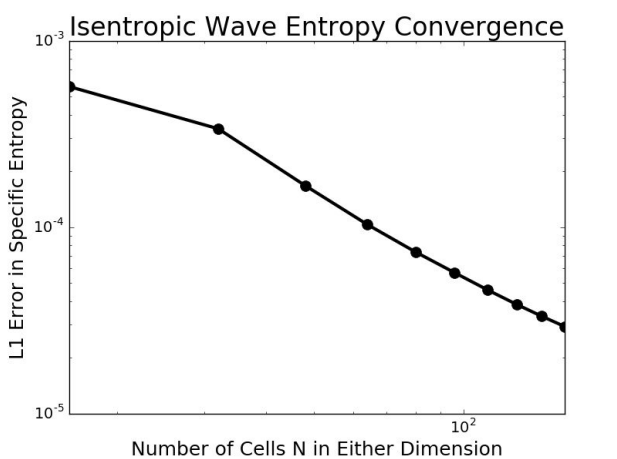
\includegraphics[width=0.75\textwidth]{figConv.png}
     \caption{Convergence plot of entropy for the isentropic wave}
     \label{f:conv}
 \end{figure}
 
\section{Acoustic Wave Simulation}
The acoustic Bessel waves were simulated by having one side (the $y=0$ side) of ghost cells in the simulation have pressure that changed as it would for a Bessel function along that side. The Bessel function describes the intensity of the wave, and acoustic intensity is proportional to the square of the pressure in the medium, so I approximated a Bessel wave incident on one side of the region by assigning a pressure $$ P(x) = P_0 + P_A \cos(\omega t)\sqrt{j_0(k_x x)} $$ for $P_0=P_A = 1$, $\omega = 2 \pi$, and $k_x = 10$, in a box spanning $-0.5 \leq x \leq 0.5$ and $ 0 \leq y \leq 5$.

The density of the system after the first wavefront just finished propagating through the system is shown in Figure \ref{f:bess1}. The streamplot at the same time is in Figure \ref{f:bess2}. 

The streamplot shows that, while the fluid at $x=0$ tends to move in the same direction as the high pressure wavefront, and moves in the negative $y$ direction only as the low pressure wavefront forms, that there are zones to the left and right of $x=0$ for which the velocity is consistently oriented in the negative $y$ direction. This seems to be a form of acoustic tweezing, since the wave is always being generated at $y=0$ and propagating upward, while the fluid is moving toward the source in those regions.  The velocity streamplot at any timestep has this behavior of a downward velocity near the pressure nodes on either side of the central peak of the wave, suggesting that a particle placed near there would drift toward the closer pressure node and move downward without ever moving in the direction of wave propagation.
 \begin{figure}
     \centering
     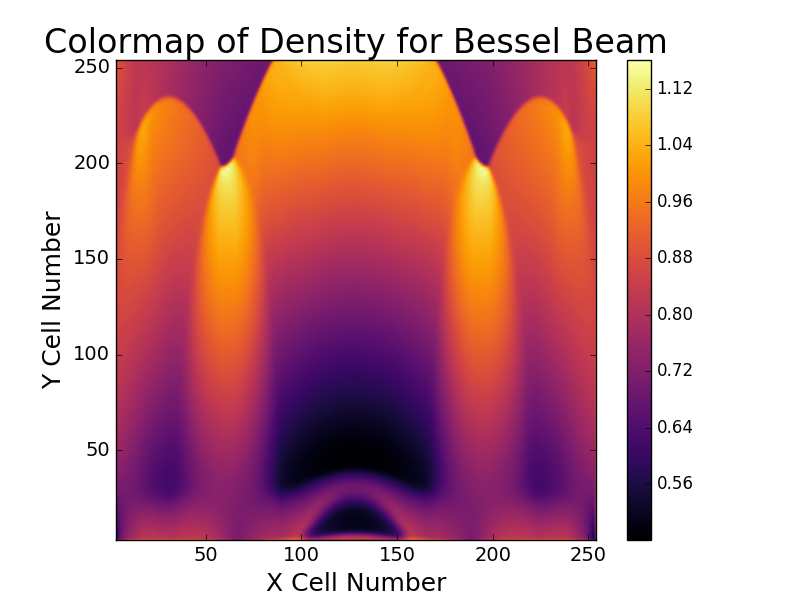
\includegraphics[width=0.75\textwidth]{bess1.png}
     \caption{Density plot of the Bessel wave near the end of the first completed propagation}
     \label{f:bess1}
 \end{figure}
 
  \begin{figure}
     \centering
     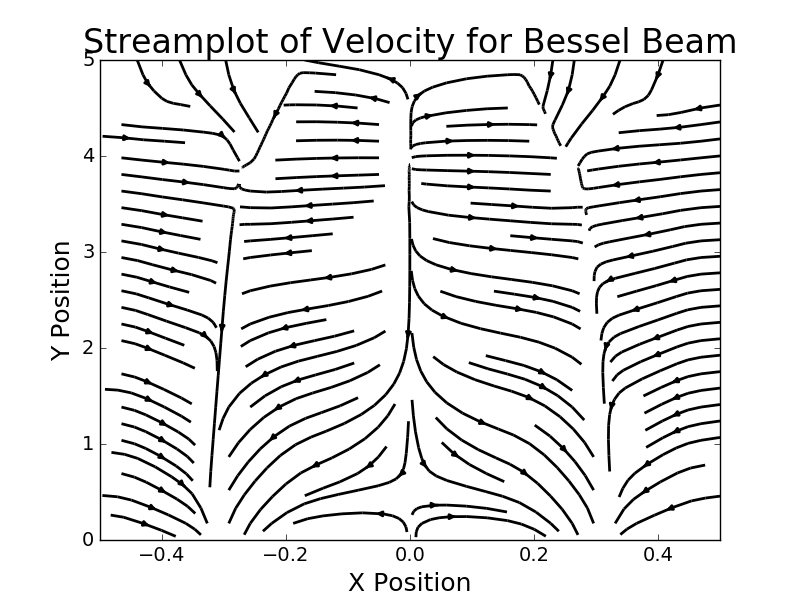
\includegraphics[width=0.75\textwidth]{bess2.png}
     \caption{Velocity plot of the Bessel wave near the end of the first completed propagation. Zones can be seen on either side of the primary peak in which the velocity flow is toward the source, rather than away from it.}
     \label{f:bess2}
 \end{figure}
\section{Future Work and Extensions}
At the moment, it becomes unfeasible to run simulations of resolution greater than around $200 \times 200$ for most cases. A $256 \times 256$ resolution run of the Bessel wave's propagation took over $4$ hours to complete. For this reason, it could be useful to parallelize the code so that higher resolutions and shorter run times can be achieved.

In addition, the simulation of an object in the fluid that could diffract the acoustic waves would be useful for studying the acoustic tweezing phenomenon that was the initial goal. However, more can be done with studying acoustic tweezing as observed in the simulations run already, such as checking whether the fluid having regions of velocity flowing toward the source is unique to Bessel waves, and what conditions could be modified to make the effect stronger and more focused. 
\end{document}
